

\tikzset{every picture/.style={line width=0.75pt}} %set default line width to 0.75pt        

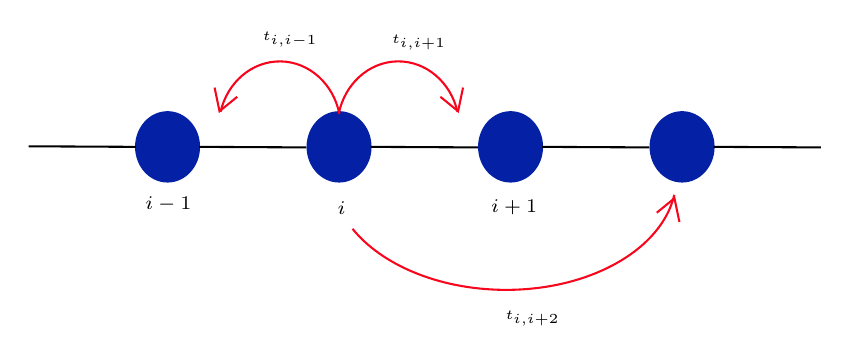
\begin{tikzpicture}[x=0.75pt,y=0.75pt,yscale=-1,xscale=1]
%uncomment if require: \path (0,221); %set diagram left start at 0, and has height of 221

%Shape: Ellipse [id:dp7587419155503419] 
\draw  [color={rgb, 255:red, 4; green, 33; blue, 166 }  ,draw opacity=1 ][fill={rgb, 255:red, 4; green, 33; blue, 166 }  ,fill opacity=1 ] (229.83,89.52) .. controls (229.83,80.3) and (236.61,72.82) .. (244.99,72.82) .. controls (253.36,72.82) and (260.15,80.3) .. (260.15,89.52) .. controls (260.15,98.75) and (253.36,106.22) .. (244.99,106.22) .. controls (236.61,106.22) and (229.83,98.75) .. (229.83,89.52) -- cycle ;
%Straight Lines [id:da47154329094458414] 
\draw    (260.15,89.52) -- (311.87,89.79) ;
%Shape: Ellipse [id:dp20440862757707068] 
\draw  [color={rgb, 255:red, 4; green, 33; blue, 166 }  ,draw opacity=1 ][fill={rgb, 255:red, 4; green, 33; blue, 166 }  ,fill opacity=1 ] (312.46,89.52) .. controls (312.46,80.3) and (319.25,72.82) .. (327.62,72.82) .. controls (335.99,72.82) and (342.78,80.3) .. (342.78,89.52) .. controls (342.78,98.75) and (335.99,106.22) .. (327.62,106.22) .. controls (319.25,106.22) and (312.46,98.75) .. (312.46,89.52) -- cycle ;
%Straight Lines [id:da43586661916081626] 
\draw    (342.78,89.52) -- (394.5,89.79) ;
%Shape: Ellipse [id:dp5119035450631295] 
\draw  [color={rgb, 255:red, 4; green, 33; blue, 166 }  ,draw opacity=1 ][fill={rgb, 255:red, 4; green, 33; blue, 166 }  ,fill opacity=1 ] (395.09,89.52) .. controls (395.09,80.3) and (401.88,72.82) .. (410.25,72.82) .. controls (418.63,72.82) and (425.41,80.3) .. (425.41,89.52) .. controls (425.41,98.75) and (418.63,106.22) .. (410.25,106.22) .. controls (401.88,106.22) and (395.09,98.75) .. (395.09,89.52) -- cycle ;
%Straight Lines [id:da8430291272192498] 
\draw    (425.41,89.52) -- (477.14,89.79) ;
%Shape: Ellipse [id:dp3949013572418896] 
\draw  [color={rgb, 255:red, 4; green, 33; blue, 166 }  ,draw opacity=1 ][fill={rgb, 255:red, 4; green, 33; blue, 166 }  ,fill opacity=1 ] (477.73,89.52) .. controls (477.73,80.3) and (484.52,72.82) .. (492.89,72.82) .. controls (501.26,72.82) and (508.05,80.3) .. (508.05,89.52) .. controls (508.05,98.75) and (501.26,106.22) .. (492.89,106.22) .. controls (484.52,106.22) and (477.73,98.75) .. (477.73,89.52) -- cycle ;
%Straight Lines [id:da6852651577323936] 
\draw    (508.05,89.52) -- (559.77,89.79) ;
%Straight Lines [id:da11908398319561075] 
\draw    (178.1,89.25) -- (229.83,89.52) ;
%Shape: Arc [id:dp6374038234551697] 
\draw  [draw opacity=0] (270.53,72.67) .. controls (273.78,58.52) and (285.57,48.13) .. (299.48,48.35) .. controls (313.38,48.56) and (324.89,59.3) .. (327.77,73.53) -- (299.06,80.54) -- cycle ; \draw  [color={rgb, 255:red, 248; green, 3; blue, 28 }  ,draw opacity=1 ] (270.53,72.67) .. controls (273.78,58.52) and (285.57,48.13) .. (299.48,48.35) .. controls (313.38,48.56) and (324.89,59.3) .. (327.77,73.53) ;  
%Shape: Arc [id:dp8860903050563039] 
\draw  [draw opacity=0] (384.7,72.67) .. controls (381.46,58.51) and (369.67,48.12) .. (355.76,48.34) .. controls (341.87,48.56) and (330.36,59.3) .. (327.47,73.53) -- (356.18,80.54) -- cycle ; \draw  [color={rgb, 255:red, 248; green, 3; blue, 28 }  ,draw opacity=1 ] (384.7,72.67) .. controls (381.46,58.51) and (369.67,48.12) .. (355.76,48.34) .. controls (341.87,48.56) and (330.36,59.3) .. (327.47,73.53) ;  
\draw  [color={rgb, 255:red, 247; green, 7; blue, 29 }  ,draw opacity=1 ] (278.56,65.4) -- (270.03,72.36) -- (267.65,60.96) ;
\draw  [color={rgb, 255:red, 247; green, 7; blue, 29 }  ,draw opacity=1 ] (376.45,65.4) -- (384.98,72.36) -- (387.35,60.97) ;
%Shape: Arc [id:dp9818262724976548] 
\draw  [draw opacity=0] (489.13,112.66) .. controls (483.04,139.07) and (448.18,158.97) .. (406.4,158.41) .. controls (375.05,157.98) and (347.94,146.13) .. (334.13,129.02) -- (407.22,103.84) -- cycle ; \draw  [color={rgb, 255:red, 247; green, 7; blue, 29 }  ,draw opacity=1 ] (489.13,112.66) .. controls (483.04,139.07) and (448.18,158.97) .. (406.4,158.41) .. controls (375.05,157.98) and (347.94,146.13) .. (334.13,129.02) ;  
\draw  [color={rgb, 255:red, 247; green, 7; blue, 29 }  ,draw opacity=1 ] (480.69,121.26) -- (489.22,114.3) -- (491.6,125.7) ;

% Text Node
\draw (325.47,114.64) node [anchor=north west][inner sep=0.75pt]  [font=\scriptsize]  {$i$};
% Text Node
\draw (399.43,113.57) node [anchor=north west][inner sep=0.75pt]  [font=\scriptsize]  {$i+1$};
% Text Node
\draw (232.75,112.17) node [anchor=north west][inner sep=0.75pt]  [font=\scriptsize]  {$i-1$};
% Text Node
\draw (351.71,34) node [anchor=north west][inner sep=0.75pt]  [font=\tiny]  {$t_{i,i+1}$};
% Text Node
\draw (406.38,167.06) node [anchor=north west][inner sep=0.75pt]  [font=\tiny]  {$t_{i,i+2}$};
% Text Node
\draw (289.42,32.6) node [anchor=north west][inner sep=0.75pt]  [font=\tiny]  {$t_{i,i-1}$};


\end{tikzpicture}

